\cotefile{147}
\scanpage{132}
\mspage{65}
contre il y en a entre $\Pi_{d,d'}$ et $\Pi_d$.
Précisons ce point, en considérant un
morphisme
\[
(215)\qquad\Delta_r\xrightarrow{\alpha}\Delta_{r'}\qquad\text{\uuline{tel que}}\quad\alpha(0)=0
\]
alors $D_{\Delta_{r'}}\longrightarrow D_{\Delta_r}$ est un morphisme
étale fini, donc aussi $D^*_{\Delta_{r'}}\unsure{\text{---}|\longrightarrow}D^*_{\Delta_r}$ induit
au dessus de $D^*_{\Delta_r}$) donc on trouve
un diagramme $2$-cartésien (qui \deleted{\unsure{suit|vient}} \inserted{peut}
\deleted{(209)} aussi se déduire de (209)
\diagram{\begin{tikzcd}[ampersand replacement=\&,column sep=large,row sep=large]
\&\widetilde\Pi_{\Delta_{r'}}\arrow[r]\arrow[d]\&\widetilde\Pi_{\Delta_r}\arrow[d]\\
(216)\&\Pi_{\Delta_{r'}}\arrow[r]\&\Pi_{\Delta_r}\arrow[ul,phantom,"2\text{-cart.}" description]
\end{tikzcd}}
)
\margin{Ceci montre que
les $\widetilde\Pi_{\Delta_r}\longleftarrow\Pi_{\Delta_r}$
et $\widetilde\Pi\unsure{\text{---}|\longrightarrow}\Pi$ sont
connus quand on
connaît les $\widetilde\Pi_d\longrightarrow\Pi_d$,
\unsure{des projections locales},
\deleted{\illegible{2}}
\uline{et} les \deleted{$\unsure{\Pi_d|P_d}$} \unsure{comme}
sur \deleted{$\unsure{\Pi_d|P_d}\longrightarrow\unsure{G_d|\Pi_d}$}
$D_d^{*!}$ sur $D_d$
\deleted{$\unsure{D_d}\longrightarrow\unsure{D^*_{\Delta_r}}$}}
où les flèches horizontales induisent sur
les $\pi_1$ des applications injectives à
image d'indice fini (on peut dire que
$\Pi_{\Delta_{r'}}\unsure{\text{---}|\longrightarrow}\Pi_{\Delta_r}$ fait de $\Pi_{\Delta_{r'}}$ un
rev. fini de $\Pi_{\Delta_r}$).

Toutes ces relations sont encore de
nature essentiellement formelle et triviale,
et marcheraient dans un site quelconque,
sans l'hypothèse spécifique des croisements
normaux, et sans que le remplacement des
\margin{131}

\scanpage{133}
$D_{\Delta_r}$ par les $D^*_{\Delta_r}$, pour définir les
$\Pi_{\Delta_r}$ et $\widetilde\Pi_{\Delta_r}$, \inserted{semble y}
jouer\deleted{\unsure{a|ait}} un rôle particulier.
\inserted{et.}

Pour \uline{$d_0$ fixé}, les systèmes
\diagram{\begin{tikzcd}[ampersand replacement=\&]
\widetilde\Pi_{d_0d_1-d_r}\arrow[r,no head]\&\Pi_{d_0,-d_r}
\end{tikzcd}}
\unsure{forment|font} un hom de groupoïdes semi-
simpliciaux, mais de nature \unsure{essentiellement}
triviale (il faudrait cepend.t examiner
à l'occasion de plus près cette soi-disant
trivialité. -- \unsure{?} elle s'explicite sans peine
en termes de la théorie de Galois
des revêtements de $D^*_{d_0}$ resp. de $P^*_{d_0}$ ...).

Nous allons maintenant introduire
un élément de structure tout à fait
non-formel, qui ne peut s'obtenir
qu'avec des hypothèses \unsure{de voisinages}
d'intersection normale, et s'exprimant
par le fait que les $\widetilde\Pi_{\Delta_r}$ (NB et
non les $\Pi_{\Delta_r}$ !) forment un groupoïde
$1/2$ simplicial, pour $\Delta_r$ variable. En d'autres
\margin{132}

\scanpage{134}
\mspage{66}
termes, il faut introduire, \deleted{\unsure{des cas}}
pour un morphisme
\diagram{\( (218) \)\qquad\begin{tikzcd}[ampersand replacement=\&]
\Delta_r\arrow[r,no head,"\alpha"]\&\Delta_{r'}
\end{tikzcd}},
un \uline{morphisme correspondant} de groupoïdes
\diagram{\( (219) \)\qquad\fbox{\begin{tikzcd}[ampersand replacement=\&]
\widetilde\Pi_{\Delta_{r'}}\arrow[r,"\widetilde\alpha^*"]\&\Pi_{\Delta_r}
\end{tikzcd}}}
qu'on appellera l'\uline{hom de générisation}
\margin{\figure{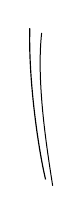
\begin{tikzpicture}[x=1cm,y=1cm]
\draw[line width=.42pt] (0,2) .. controls (-.02,1.38) and (.10,.50) .. (.20,.08);
\draw[line width=.36pt] (.15,1.94) .. controls (.08,1.31) and (.22,.45) .. (.29,0);
\end{tikzpicture}}}
associé à $\alpha$. Comme $\alpha$ se factorise
canoniquement en un hom surjectif
suivi d'un hom injectif de simplexes,
on est ramené à examiner séparément
les deux cas. Mais si $\alpha$ est surjectif
(``hom de dégénérescence''), \deleted{l'homomorphisme}
\inserted{on a $\alpha(0)=0$}
donc on est dans le cas déjà envisagé --
\deleted{\unsure{correspondant}}\inserted{d'ailleurs} dans ce cas
\diagram{\begin{tikzcd}[ampersand replacement=\&]
D^*_{\Delta_{r'}}\arrow[r]\&D^*_{\Delta_r}
\end{tikzcd}}
\unsure{se}
décompose en des morphismes \unsure{:|;}
\diagram{\( (220) \)\qquad\begin{tikzcd}[ampersand replacement=\&]
D^*_{d'_0,-\,-,d'_{r'}}\arrow[r]\&D^*_{\unsure{d_0^{\deleted{\prime}}|d'_0},-\,-,\unsure{d_r^{\deleted{\prime}}|d'_r}}
\end{tikzcd}},
$(d_0,-\,-,d_r)$ est déduite de $(d'_0,-,d'_r)$
en \unsure{réécrivant} cette suite, en répétant certains
de ses éléments -- et \deleted{les} alors (220) est
un iso -- donc \uline{si $\alpha$ est un hom}
\margin{On voit que la
considération des
$\widetilde\Pi_{d_0-d_r}$, $\Pi_{d_0,-d_r}$
pour $d_0,-\,-,d_r$ non
\uline{strictement} \unsure{décroissants|décroiss.}, et
celle de $\alpha^*$, pour $\alpha$ \unsure{non}
\uline{stricts} \unsure{croissants|croiss.}, est de
la poudre aux yeux
simplement !}
\margin{133}

\scanpage{135}
\uline{de dégénérescence}, \uline{alors} (219) \uline{est un}\deleted{e}
\deleted{\unsure{équiv.}}\uline{isomorphisme}, de nature ess.\textsuperscript{t} triviale.

On est donc réduit à regarder le
cas d'une application \uline{injective} $\alpha$ (``opération
face''), et le \inserted{seul} cas qui \deleted{\unsure{pose}} pose problème
est bien sûr celui où $\alpha(0)\ne0$. Donc
\[
\tag{221}
\left\{\begin{aligned}
d_*&=\{d_0>d_1\mathinner{\cdot\,{-}\,{-}}>d_r\},\quad\text{et si}\\
d'_*&=\{d'_0>d'_1>\mathinner{\cdot\,{-}}>d'_{r'}\}\text{ est }
\text{\deleted{\unsure{une sous-suite}}}\inserted{\text{contenu dans }d_*},
\end{aligned}\right.
\]
\[
d'_0\ne d_0\text{ ie. }d'_0<d_0,\quad\text{il faut}
\]
définir l'hom
\[
(222)
\]
\diagram{\begin{tikzcd}[ampersand replacement=\&]
\Pi_1P^*_{d_0\deleted{\unsure{\geq}}d_1,\mathinner{{-}\,{-}},d_r}\arrow[r]\&
\Pi_1P^*_{d'_0,\mathinner{-},d'_r}
\end{tikzcd}}
\margin{attention, on a subrepticement chang\unsure{é}
de notations, en interver-tissant $d_*$ et $d'_*$ !}
\margin{on se réduit au cas
de $d_0,d_1,\mathinner{-},d_r$ strict.\textsuperscript{t}
\unsure{décroissant|décroissants} -- auquel on
parvient aussitôt. --
En fait, on est ramené au cas où $r'=r-1$, et où il
s'agit de l'opération ``face de codim $1$'' pour laquelle
$\alpha(0)\ne0$, donc correspondant :
\diagram{\begin{tikzcd}[ampersand replacement=\&]
D_{d_0,d_1,\mathinner{-},d_r}\arrow[r]\&D_{d_1,\mathinner{{-}\,{-}},d_r}
\end{tikzcd}}}

Notons que l'on a
\[
(223)
\]
\diagram{\begin{tikzcd}[ampersand replacement=\&]
D^{\deleted{*}}_{d_0,\mathinner{{-}\,{-}},d_r}\arrow[r]\&D_{d'_0,\mathinner{-},d'_{r'}}
\end{tikzcd}}
(mais \uline{non} un morphisme entre les
espaces avec $*$ !), qui est une immersion \inserted{locale}
d'espaces analytiques lisses, de codim
$d_0-d'_0$, \deleted{qui}\inserted{\unsure{ainsi|et}} s'insère dans le diagramme
\margin{134}

\scanpage{136}
\mspage{67}
\[
(22\unsure{4})
\]
\diagram{\begin{tikzcd}[ampersand replacement=\&]
D_{d_0,\text{--},d_r}\arrow[r]\arrow[d]\&D_{d'_0\,\cdot\,\text{--}\,d'_{r'}}\arrow[d,harpoon,"\unsure{}" description]\\
D_{d_0,d'_0}\arrow[r]\&D_{d'_0}^{\deleted{\unsure{*}}}
\end{tikzcd}}
où les flèches verticales sont étales,
et la $2^{\mathrm{ième}}$ flèche horizontale est une
immersion locale de codim $d_0$ \deleted{$-d'_0$. \unsure{On a}}
\[
(225)\qquad \unsure{d|\delta}=d_0-d'_0
\]
[Dans le typique (auquel on se réduit)
où $\unsure{\deleted{\{}}d'_* = \{\unsure{\uline{d_1}}>\cdot\,\text{--}>d_r\}$, le diagramme
(224) est cartésien -- \deleted{\unsure{comme on voit}}\inserted{plus génér.\textsuperscript{t}}, il
\unsure{reste} \deleted{\unsure{tjs}} cartésien, \inserted{si $d'_0=d_1$} et c'est trivial.]
\margin{\uline{NB} Dans le cas général, on a
\diagram{\begin{tikzcd}[ampersand replacement=\&, column sep=small]
D_{d_*}\arrow[r,"{\text{fini \unsure{étale|étal}}}"']\arrow[dd,dotted]\&D_{\widetilde d'_*}\arrow[r]\arrow[d]\&D_{d'_*}\arrow[d]\\
\&D_{d_0,d'_0}\arrow[dl,dotted]\arrow[r]\&D_{d'_0}\\
D_{d_0}\&\&
\arrow[ul,phantom,from=2-3,to=1-2,"{\text{cart}}" description]
\end{tikzcd}}}
Considérons le morphisme induit
\[
(225)\qquad D^*_{d_*}\longrightarrow D_{d'_*}
\]
(Attention, on a mis un $*$ en exposant
à $D_{d_*}$ \unsure{seulem\textsuperscript{t}|seulemen\textsuperscript{t}}, non : $D_{d'_*}$ !).

Nous munissons $D_{d'_*}$ du diviseur
$\Theta_{d'_*}$ image inverse de $\Theta_{d_0}$ sur $D_{d_0}$.
On désigne par $\Theta_{d'_*}^{(p)}$ le ``squelette
de dim $p$'' de $\Theta_{d'_*}^{p}$, et \deleted{\unsure{p}} on pose
\margin{135}

\scanpage{137}
\[
\tag{226}
\Theta_{d'_*}^{\unsure{d|\delta}*}\overset{\mathrm{def}}=
\Theta_{d'_*}^{\unsure{d|\delta}}\setminus
\Theta_{d'_*}^{\unsure{d+1|\delta+1|d1}}
\]
squelette \unsure{``privé''|purifié|ponctué}
de codim. $d$ de
$\Theta_{d'_*}$ dans $D_{d'_*}$.

Ceci posé, on voit que $225$ \unsure{\deleted{est}}\inserted{induit}
un \deleted{morphisme} iso\uline{morphisme local}
\uline{de} $D_{d_*}$ \uline{sur} \deleted{$\unsure{D|\Theta}_{d'_*}$} $\Theta_{d'_*}^{d*}$. Plus
précisément, \deleted{$\Theta_{d'_*}^{d\unsure{*|\deleted{*}}}$ s'identifie}
\inserted{\unsure{à}} \deleted{:}
\deleted{$D_{(d_0,d'_0,-,d'_r)}\ \unsure{:}\ D_{\widetilde d'_*}$, \unsure{où}}
\[
(22\deleted{\unsure{6}}7)\qquad
\Theta_{d'_*}^{(d)}\xleftarrow{\ \sim\ }D_{\widetilde d'_*}
\]
où \deleted{$d'$\unsure{,}}
\[
\widetilde d'_*=(d_0,d'_0,-\,-,d'_r)
\]
et cet isom. induit un isom
\[
(228)\qquad
D_{\widetilde d'_*}^{*}\xrightarrow{\ \sim\ }\Theta_{d'_*}^{(d)*},
\]
d'autre part (223) $D_{d_*}\mathrel{\text{---}}D_{d'_*}$ se
factorise en
\[
(229)
\]
\diagram{\begin{tikzcd}[ampersand replacement=\&,row sep=large]
D_{d_*}\arrow[r,no head]\&D_{\widetilde d'_*}\arrow[r]\arrow[d,phantom,"{\begin{tikzpicture}[baseline=(v.base)]\node[rotate=90,inner sep=0pt] (v) {$\simeq$};\end{tikzpicture}}" description]\&D_{d'_*}\\
\&\Theta_{d'_*}^{(d)\unsure{*|\deleted{*}}}\&
\end{tikzcd}}
donc c'est un morphisme étale fini,
suivi \inserted{\unsure{est|du}} \unsure{\deleted{d'}|d'}un morphisme d'inclusion de
$\Theta_{d'_*}^{(d)}$ dans $D_{d'_*}$. De plus, comme $D_{d_*}^{*}$ est
\margin{136}

\cotefile{148}
\scanpage{2}

\margin{(29.11.83)}

Soit $X$ surf. à bord compacte orientée, à structure torique
\inserted{(i.e. torseur sous $\mathbb U=\{z\in\mathbb C\mid |z|=1\}$\unsure{)}}
donnée sur les comp. connexes du bord.
On définit
\[
\begin{aligned}
\operatorname{SRT}(\unsure{\deleted{X}|X})={}&
\text{quotient du groupe des }\text{autom de }X
\text{ (}\text{\deleted{\unsure{en}} resp. }\text{l'orientation}\\
&\text{et les structures toriques) }\text{par la comp. neutre du}\\
&\text{sous-groupe }\operatorname{Aut}^!(\vec X)
\deleted{\unsure{\mathrm{bijec.}}}
\text{ de Aut }\text{qui induit}\\
&\text{l'identité sur }\partial X
\end{aligned}
\]

On a ainsi un dévissage de $\operatorname{SRT}(X)$ en trois étages
\[
\underbrace{S_{\unsure{*}}T^!(X)}_{
\operatorname{Aut}^!(\unsure{\vec X|\overline X})/\text{comp. neutre}}
\qquad\mathbb U^I\qquad\mathfrak S_I
\qquad I=\pi_0(\partial X)
\]
ou encore
\[
\mathbb Z^I\qquad T(X)\qquad\mathbb U^I\qquad\mathfrak S_I
\]

En fait, on définit can! un sous-groupe \inserted{droit}
$\mathbb R^I$ de $\operatorname{SRT}(X)$
contenant $\mathbb Z^I$, de telle façon qu'on ait
\[
\underbrace{\operatorname{SRT}^!(X)}_{
\substack{\text{noyau de}\\
\operatorname{SRT}^!(\alpha)\to\mathfrak S_I'}}
=\mathbb R^I.S_{\unsure{*}}T^!(X)
\]

\margin{\deleted{\unsure{et propre}}}
\diagram{
\begin{tikzcd}[column sep=small,row sep=small]
\mathbb R^I\arrow[dd,"\text{cocart}"{pos=.65,right}] &
\mathord{:}\arrow[l,phantom,"\unsure{\leftharpoonup}" description] &&\\
&&\unsure{\deleted{\lambda}|\lambda}&\\
\mathbb Z^I\arrow[r,hook]&
S_*T^!\arrow[uu,hook]\arrow[r,phantom,"\subset"]&
\operatorname{SRT}^!\arrow[r,phantom,"\subset"]&
\operatorname{SRT}
\end{tikzcd}
}

i.e. on a

\margin{\hfill$\unsure{*}$\par
\uline{NB} $\operatorname{SUT}(X)\simeq
T(X)\times_{\mathfrak S_I}\operatorname{Aut}((T_i)_{i\in I})$}

\margin{jusqu'ici on ne fait intervenir
que $S_*T^!(X)$; à l'exclusion de $S_*T(X)$,
dont la défini. exige une str. suppl.
$\uline{s}$, cf ci-dessous}

\diagram{
\begin{tikzcd}[column sep=small,row sep=large]
&\operatorname{SRT}(X)\arrow[d,no head,"\mathfrak S_I"]&\\
&\mathbb R^I.S_{\unsure{*}}T^!\arrow[dl,no head,"T^!"']
 \arrow[dr,no head,"\mathbb U^I"]&\\
\mathbb R^I\arrow[dr,no head,"\mathbb U^I"']&&S_*T^!(X)\\
&\mathbb Z^I\arrow[ur,no head,"T^!(X)"']&
\arrow[from=1-1,to=2-1,phantom,"\Bigg\{" description,"T(X)"']
\arrow[from=1-3,to=2-3,phantom,"\Bigg\}" description,"\operatorname{Aut}((T_i)_{i\in I})"]
\end{tikzcd}
}

d'où
\diagram{
\begin{tikzcd}[row sep=large,column sep=small]
\operatorname{SRT}\deleted{(X)}/\mathbb Z^I
 \overset{\text{déf}}=\operatorname{SUT}(X)
 \arrow[d,phantom,"\unsure{\downharpoonright|\downarrow}" description]&\\
T^!(X)\times\mathbb U^I&
\arrow[from=1-2,to=2-2,phantom,"\Bigg\}" description,"\mathfrak S_I"]
\end{tikzcd}

\begin{tikzpicture}[x=1cm,y=1cm]
\draw[line width=.25pt] (0,0) .. controls (.35,-.04) and (.66,-.04) .. (.91,-.01);
\draw[line width=.25pt] (.94,-.01) .. controls (1.07,-.01) and (1.13,.02) .. (1.19,.01)
 .. controls (1.23,-.07) and (1.3,-.07) .. (1.45,-.05)
 .. controls (1.78,-.03) and (2.06,.04) .. (2.25,.05);
\draw[line width=.25pt] (2.31,.04) .. controls (2.57,-.02) and (2.91,-.09) .. (3.17,-.06)
 .. controls (3.43,-.04) and (3.64,.01) .. (3.81,.07);
\draw[line width=.25pt] (3.94,.08) .. controls (4.16,.1) and (4.38,.04) .. (4.63,.04);
\end{tikzpicture}
}
\[
(*)\qquad1\longrightarrow\mathbb U^I\longrightarrow
\operatorname{SUT}(X)\longrightarrow\unsure{T}(X)-1
\]

De plus, chaque fois qu'on se donne un
marquage, i.e. un pt \deleted{\unsure{de}}
\[
\uline{s}=(s_i)\in
\prod_{i\in I=\pi_0(\partial X)}
\deleted{\unsure{(\mathbb U_i)}}T_i
\]
\margin{$T_i=$ comp. connexe (torique) de $\partial X$ d'indice $i$}

on trouve un plongement
\[
S_*T^{\deleted{\unsure{!}}}(X,\uline{s})\hookrightarrow\operatorname{SRT}(X)
\]
tel qu'on en déduise
\[
S_*T^{\deleted{\unsure{!}}}(X,\uline{s})
\mathbin{\wedge}_{\mathbb Z^I}\mathbb R^I
\simeq\operatorname{SRT}(X)
\]

\margin{1}

\scanpage{3}

Une façon de le voir est de dire que
la donnée de $\uline{s}$ définit un scindage
\inserted{$\varphi_{\uline{s}}$} de
l'extension $(*)$ ci-dessus, et que \unsure{vu} pour
ss-groupe de $\operatorname{SRT}(X)$,
$S_1T(X,\uline{s})$ s'identifie
\unsure{:|à} l'image inverse de
\[
\varphi_{\uline{s}}(T(X))\subset\operatorname{SUT}(X)
\]
par l'hom. can
\[
\operatorname{SUR}(X)\unsure{\longrightarrow}\operatorname{SUT}(X)
\]
de passage au quotient. Le chgt de
$\uline{s}$ en $\uline{s}'=u.\uline{s}$
transforme $\varphi_{\uline{s}}$ en
\[
\varphi_{\uline{s}'}=\operatorname{int}(u)\circ\varphi_{\uline{s}}
\]
donc (si $\widetilde u\in\mathbb R^I$ relève $u$, on trouve
\[
S_1T(X,\uline{s}')
=\operatorname{int}(\widetilde u)S_1T(X,\uline{s}).
\]

En termes de $\unsure{\overline X|\vec X}$, la définition de
$S_1T(X,\uline{s})$
dépend un choix $\uline{s}$ \uline{non-anodin},
par contre celle de $S_1RT(X)$ ne dépend que d'
un choix anodin, celui de la famille des
structures toriques $(t_i)_{i\in I}$.
De plus $\prod T_i$ comme
torseur sous $\unsure{\mathbb U^I}$ se réalise
\inserted{(pas fidèlement d'ailleurs)}
comme \unsure{une classe} de scindages de l'ext. $(*)$
(via autom. int. par $\mathbb U^I$)
$\bigl[$déduit\unsure{s} de $\operatorname{SRT}(X)$
avec \unsure{ses|les} structures suppl.$\unsure{\}|]}$
savoir) les inclusions

\diagram{
\begin{tikzcd}[row sep=small]
\mathbb R^I\arrow[dr] &\\
&\operatorname{SRT}(X)\\
S_1T^!(X)\arrow[ur]&
\end{tikzcd}
}

coïncidant sur $\mathbb Z^I$.

\margin{2}

\scanpage{4}

Ceci dit, si on se donne un
multimarquage de $\partial X$, savoir pour
chaque $i\in I$ un $n_i\in\mathbb N^*$ et un
sous-\inserted{\unsure{$\mathbb Z/n_i$|$\mathbb Z_{n_i}$}-}torseur $T_i(n_i)\subset T_i$, \deleted{\unsure{de groupe|les groupes}} i.e
un $s_i\in T_i^{\wedge n_i}$, d'où $\deleted{\uline{s}\unsure{\in}}$
\[
\uline{s}\in\prod_{i\in I}T_i^{\wedge n_i},
\]
alors le groupe de Teichm\unsure{ü|u}ller multimarqué
$S_{\unsure{*|1}}T(\unsure{X},\uline{s})$, généralisant le précédent, est
plongé dans $\operatorname{SRT}(X)$ de façon naturelle,
en prenant un $s_i^0$ dans chaque $T_i(n_i)$, d'où
$\uline{s}^0\in\prod T_i$ et $ST(X,\uuline{s}^0)\subset\operatorname{SRT}(X)$, et on
prend le ss-groupe
\[
ST(X,\uline{s})=ST(X,\uline{s}^0).\prod_{i\in I}\frac1{n_i}\unsure{\mathbb Z_i;|\mathbb Z_{i_i}}
\]
où $\mathbb Z_i$ est le $i$ème facteur de $\mathbb Z^I\subset\operatorname{SRT}(X)$.

\margin{3}

\scanpage{5}
\mspage{1}

\uline{Courbes} \inserted{exceptionnelles} \uline{de type} $(1,1)$ (sur $\mathbb C$)

A) \uline{Courbe} \inserted{ell.} \uline{anharmonique de type carré}

Cat. de ces courbes équivalente : celle des carrés
\unsure{com}binatoires orientés, i.e. des torseurs sous
\[
\mathbb Z/4\mathbb Z\simeq\mu_4(\mathbb C)\simeq\text{groupe des unités algébriques de }\mathbb Q[i]
\]
\margin{i.e. groupe des unités de $\mathbb Z[i]$ (\unsure{ann}eau des entiers de $\mathbb Q[i]$}

La donnée d'un tel torseur \inserted{$S$} permet de tordre
$\mathbb E\ell_0\overset{\mathrm{def}}\simeq\mathbb C/\mathbb Z[i]$ et trouver
\[
\mathbb E\ell_0(S)\simeq\mathbb E\ell_0\mathbin{\wedge}_{\mathbb Z/4\mathbb Z}S
\]

\margin{\figure{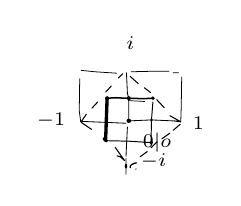
\begin{tikzpicture}[x=.006cm,y=-.006cm,line cap=round,line join=round] \draw[line width=.28pt] (60,72)--(89,75)--(135,78) (166,75)--(207,74)--(246,74) (255,77)--(266,77); \draw[line width=.28pt] (57,90)--(56,158)--(59,180) (273,86)--(272,149)--(271,180); \draw[line width=.38pt] (148,79)--(139,88) (124,105)--(112,118) (95,139)--(83,152) (71,165)--(60,181); \draw[line width=.38pt] (164,85)--(181,100) (194,109)--(207,119) (220,134)--(236,151) (248,168)--(271,181) (256,179)--(271,181); \draw[line width=.38pt] (270,186)--(255,199) (248,205)--(231,217) (221,223)--(208,236) (200,244)--(185,255); \draw[line width=.38pt] (60,182)--(82,197) (132,235)--(152,263) (136,253)--(143,255)--(152,263); \draw[line width=.55pt] (115,131)--(133,130)--(154,131)--(161,131)--(192,132)--(212,131); \draw[line width=.25pt] (160,136)--(195,138); \draw[line width=1.2pt] (115,131)--(113,187)--(112,216)--(109,217)--(113,221); \draw[line width=.35pt] (212,139)--(209,177)--(208,225) (113,221)--(160,222)--(208,225); \draw[line width=.3pt] (156,77)--(158,121)--(161,131)--(161,179) (158,192)--(155,254) (155,259)--(155,292); \draw[line width=.3pt] (59,180)--(155,184) (161,179)--(209,177)--(254,179); \fill (115,131) ellipse[x radius=4.5,y radius=4.2]; \fill (161,131) ellipse[x radius=4.1,y radius=4.5]; \fill (212,131) ellipse[x radius=4.1,y radius=4.1]; \fill (161,179) ellipse[x radius=5.0,y radius=4.5]; \fill (209,174)--(212,177)--(209,181)--(206,177)--cycle; \fill (113,221) ellipse[x radius=3.8,y radius=4.0]; \fill (208,225) ellipse[x radius=4.2,y radius=3.9]; \fill (155,275) ellipse[x radius=2.7,y radius=5.0]; \node[font=\scriptsize,anchor=east] at (47,179) {$-1$}; \node[font=\scriptsize,anchor=west] at (276,183) {$1$}; \node[font=\scriptsize,anchor=south] at (164,49) {$i$}; \node[font=\scriptsize,anchor=north west] at (170,184) {$\unsure{0|o}$}; \node[font=\scriptsize,anchor=west] at (166,264) {$-i$}; \draw[line width=.48pt] (177,268) .. controls (170,269) and (162,273) .. (164,278); \fill (176,281) circle[radius=1.4]; \end{tikzpicture}}}

Si le carré est réalisé comme carré \inserted{euclidien}
dans un plan euclidien \inserted{$V_S$} (canoniquement), de centre $\unsure{0|o}$,
\figure{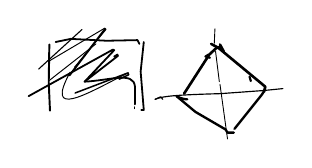
\begin{tikzpicture}[x=.008cm,y=-.008cm,line cap=round,line join=round] \draw[line width=.7pt] (40,34)--(39,94)--(41,139); \draw[line width=.65pt] (50,30)--(74,25)--(131,28)--(180,27)--(183,33); \draw[line width=.65pt] (190,30)--(185,77)--(190,138)--(186,138); \draw[line width=.4pt] (23,73)--(92,10); \draw[line width=.35pt] (40,60)--(128,8)--(130,10)--(80,70); \draw[line width=.7pt] (128,10)--(72,83); \draw[line width=.35pt] (40,91)--(114,33); \draw[line width=.65pt] (7,116)--(141,42)--(143,43)--(96,93)--(149,52)--(148,50)--(143,53); \draw[line width=.35pt] (73,78) .. controls (32,153) and (98,113) .. (161,81); \draw[line width=.55pt] (81,111)--(165,79)--(166,82)--(151,89); \draw[line width=.65pt] (96,93) .. controls (137,91) and (174,76) .. (176,101) -- (176,129); \draw[line width=.35pt] (175,133)--(175,136); \begin{scope}[shift={(200,5)}] \draw[line width=.32pt] (103,4)--(102,27) (104,40)--(110,88) (111,92)--(123,179); \draw[line width=.42pt] (8,116) .. controls (20,111) and (40,109) .. (112,107) -- (181,102)--(211,99); \draw[line width=.42pt] (8,116)--(17,112)--(20,116); \draw[line width=.95pt] (54,107)--(94,45)--(107,33) (107,33)--(183,96)--(181,104); \draw[line width=.95pt] (97,28)--(108,34) (111,29)--(117,40)--(108,33); \draw[line width=.8pt] (93,45)--(88,48)--(95,50) (158,80)--(160,87); \draw[line width=.85pt] (42,111) .. controls (49,115) and (55,116) .. (59,116); \draw[line width=.85pt] (42,111)--(72,136)--(120,164)--(123,169)--(133,169); \draw[line width=.85pt] (134,163)--(178,108)--(181,103); \end{scope} \end{tikzpicture}}
on en déduit dans le plan (vectoriel via $\unsure{0|o}$) $V_S$
un syst. de deux \deleted{\unsure{axes} de}
coordonnées \inserted{mod. signes\unsure{,}}
via les diagonales, d'où un
\deleted{\unsure{lattice}} \inserted{réseau}
$\Gamma_S$ dans $V_S$ (sous-groupe discret de
rang $2$) et
\begingroup \setbox0=\hbox{$\displaystyle \mathbb E\unsure{\ell_0(S)\,2|\ell_0(S)/2}X_S=V_S/\Gamma_{\unsure{r|\Gamma|S}}.$} \[ \rlap{\begin{tikzpicture}[overlay,x=\wd0,y=1ex,line cap=round,line join=round] \draw[line width=.35pt] (-.43,-1.0) .. controls (-.27,-1.3) and (-.08,-.9) .. (-.055,-.5) .. controls (-.05,.25) and (-.08,1.4) .. (-.10,2.1) -- (.45,2.0) -- (1.04,2.4) -- (1.07,-.7) -- (1.18,-.65); \end{tikzpicture}} \copy0 \] \endgroup

\margin{\figure{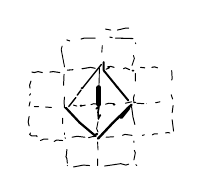
\begin{tikzpicture}[x=.006cm,y=-.006cm,line cap=round,line join=round] \draw[line width=.35pt] (182,14)--(193,16) (207,16)--(224,12)--(231,12); \draw[line width=.38pt] (100,37)--(106,39) (130,35)--(137,33)--(160,33) (191,31)--(196,32) (203,33)--(240,34); \draw[line width=.32pt] (90,50)--(88,57)--(95,94) (175,49)--(174,63) (245,43)--(246,45) (241,70)--(243,76)--(238,91); \draw[line width=.38pt] (26,105)--(31,106)--(39,104)--(48,106) (64,105)--(71,104)--(85,106) (101,101)--(113,100) (132,98)--(150,95)--(160,97); \draw[line width=.38pt] (183,99)--(190,96) (186,94)--(193,93)--(200,95) (220,98)--(224,96)--(233,100) (256,95)--(265,96) (280,95)--(286,94)--(292,96); \draw[line width=.35pt] (322,102)--(323,119)--(322,122) (321,153)--(324,162) (325,176)--(323,191) (323,206)--(326,230); \draw[line width=.35pt] (24,124)--(21,133)--(22,139) (23,151)--(21,154) (22,168)--(20,177) (20,199)--(18,211)--(20,219) (23,234)--(21,237)--(25,240)--(36,240); \draw[line width=.35pt] (94,110)--(93,133) (95,158)--(94,168)--(95,181) (91,203)--(91,214) (95,234)--(95,237) (96,244)--(97,245) (100,269)--(99,281)--(98,284)--(100,288)--(101,298); \fill (101,303) circle[radius=1.2]; \draw[line width=.35pt] (245,108)--(245,124) (243,153)--(241,160)--(242,170)--(246,169) (237,178)--(240,200)--(244,216) (242,251)--(242,254) (243,271)--(245,276)--(242,291) (246,301)--(248,303); \draw[line width=.35pt] (31,178)--(40,178) (55,179)--(67,180) (114,175)--(121,177) (129,177)--(139,175) (151,174)--(157,172)--(164,173); \draw[line width=.35pt] (182,173)--(189,171)--(200,172) (224,171)--(237,168) (248,171)--(263,172) (288,170)--(297,168); \fill (269,172) circle[radius=.7]; \draw[line width=.35pt] (37,242)--(36,240) (44,250)--(51,247)--(60,247) (73,252)--(78,249)--(91,250) (111,243)--(122,241)--(138,243) (146,244)--(153,242)--(162,241); \draw[line width=.35pt] (183,243)--(199,242) (218,239)--(223,237)--(238,239) (260,239)--(264,238) (281,238)--(285,236)--(292,236) (309,234)--(314,233)--(318,234); \draw[line width=.35pt] (114,306)--(135,302)--(148,303) (180,304)--(194,302)--(214,299)--(225,302)--(231,300); \draw[line width=.32pt] (169,97)--(168,134) (166,210)--(163,225)--(166,232) (165,253)--(166,270) (165,289)--(165,303); \draw[line width=.5pt] (173,89)--(133,139) (130,143)--(122,154) (119,159)--(104,178); \draw[line width=.7pt] (178,84)--(178,101)--(180,105) (180,104)--(206,136)--(230,165); \draw[line width=.8pt] (98,181)--(127,212)--(159,239)--(164,236); \draw[line width=.85pt] (237,174)--(197,213)--(166,246); \draw[line width=1.25pt] (231,181)--(215,201); \draw[line width=1.8pt] (168,138)--(168,173); \draw[line width=.6pt] (168,178)--(166,190)--(167,204) (162,183)--(166,179) (171,196)--(168,201); \foreach \x/\y in {132/139,206/136,127/212,197/213,169/173,130/176,200/174,240/102}{\fill (\x,\y) ellipse[x radius=3.1,y radius=2.3];} \fill (167,204) circle[radius=1.6]; \end{tikzpicture}}}

Il y a dans $X_S$ un élement\raisebox{-.6em}{\unsure{:}} d'ordre $2$ canonique
\inserted{$\eta_S$}
(stable par automorphismes), les deux autres él. d'
ordre $2$ sont échangés par le générateur $i$ de
$\mu_4(\mathbb C)\simeq\operatorname{Aut}(\unsure{X_S|X})$.
(\leavevmode\hbox{\rlap{\kern.30em\underline{\kern-.30em\phantom{NB}}}NB} $\eta_S$ \unsure{peu}t donc être \unsure{défini}

\margin{4}

\scanpage{6}

\begin{center}
U N I V E R S I T E\\
DES SCIENCES ET TECHNIQUES\\
DU LANGUEDOC\\
\textasciicircum\textasciicircum\textasciicircum\textasciicircum\textasciicircum\textasciicircum\textasciicircum\textasciicircum\textasciicircum\textasciicircum\textasciicircum\textasciicircum\textasciicircum
\end{center}

Montpellier, le 14 octobre 1983

Service de la Scolarité

Diffusion : Liste A\\
MA/gs \hfill N° 4375

\begin{center}
AVIS DE SOUTENANCE D'UNE THESE DE DOCTORAT DE 3e CYCLE

ECOLOGIE GENERALE ET APPLIQUEE OPTION ECOLOGIE AQUATIQUE\\
\texttt{========================================================}
\end{center}

\uline{NOM et Prénom du candidat} : MONTI Dominique

\uline{Titre de la thèse} : ``Recherches sur l'optimisation du plan d'échantillonnage employé pour la cartographie des peuplements benthiques. Application à la macrofaune benthique de l'étang de Pierre Blanche (Palavas, Hérault, France).

\uline{Date,-heure et lieu de soutenance prévus} : Le 2 novembre 1983 à 15 heures,\\
Salle de cours n° 9 - Université des Sciences et Techniques du Languedoc

\uline{Nom du Directeur de thèse} : M. AMANIEU

\uline{Désignation du Laboratoire où la thèse est préparée} : Laboratoire d'Hydrobiologie marine - U.S.T.L.

\uline{Analyse de l'ouvrage} : Cette réflexion porte sur le problème du choix du nombre et de l'organisation spatiale des points de prélèvement en écologie. Quel effort doit-on fournir pour un niveau de précision fixé ? Et où doit-on prélever ?

Ce travail est basé sur la réalisation de différents sous-échantillonnages d'une information initiale supposée maximale. Les différents sous-échantillonnages varient par le nombre et l'organisation spatiale des points de prélèvements ; et ils sont tous effectués à partir de la même liste d'objets.

Chaque sous-échantillonnage employé donnera naissance à une carte qui sera par la suite comparée à la carte dite ``de référence'' ; il restera à apprécier au vu de ces résultats si les cartes obtenues diffèrent de la référence, en quelles proportions et de quelle manière.

Les résultats théoriques sont appliqués à l'étude de la macrofaune benthique d'un étang littoral (l'étang de Pierre Blanche à Palavas, France).

\uline{Durée approximative des recherches ayant abouti à la thèse} : 3 ans

\uline{Composition du jury Proposé} : \begin{tabular}[t]{ll}
MM. & AMANIEU M.\\
& BLANC F.\\
& FRONTIER S.\\
& GRANDJOUAN G.\\
& LASSERRE G.
\end{tabular}

\begin{flushright}
P/ le Secrétaire Général,\\
L'Attachée Principale d'Administration\\
Scolaire et Universitaire,

\unsure{A. Gentil}

A. GENTIL
\end{flushright}

\margin{5}

\scanpage{7}
\mspage{2}

comme l'unique élément de \({}_2(X_S)\) qui est fixe par $\operatorname{Aut}(X_S)\simeq\mathbb Z/4\mathbb Z$. En fait
\inserted{\[
(X_S)^{\unsure{\deleted{i}|f}i}\overset{\mathrm{def}}{=}\{x\in X_S\deleted{\}} \mid ix\unsure{=|\simeq}x\}=\{e,\eta_S\}
\]}
\deleted{\unsure{$X$|$X_S$}} La surface top. $X_S$ a une déc. cell. \inserted{\unsure{can|ces}} avec 1 sommet $e$, deux arêtes, une face, \inserted{ces arêtes} correspondant aux deux mailles du réseau $\Gamma_S$.

On considère $X_S$ comme muni de cette décomposition. Parfois c'est l'image inv. de celle-ci par $2\operatorname{id}_{X_S}$ qui est plus commode, 4 sommets (formant \({}_2(X_S)\)), \deleted{quatre} \inserted{huit} arêtes, \deleted{(\uline{NB} \unsure{le}} \inserted{$4^{\unsure{\smallfrown}}$} faces. On peut considérer $\mathbb Z/4\mathbb Z\simeq\mu_4(\mathbb C)$ comme le groupe d'automorphismes commun de ces deux structures cellulaires.

\figure{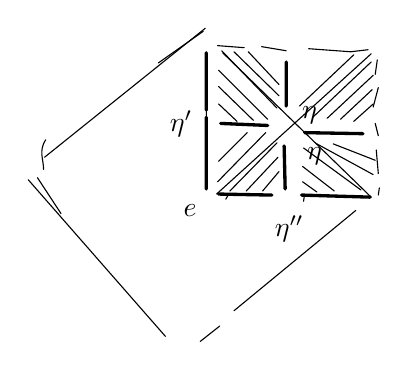
\begin{tikzpicture}[x=.013cm,y=-.013cm,line cap=round,line join=round]
\draw[thin] (-153,110)--(4,-16);
\draw[thin] (-152,93) .. controls (-159,104) and (-154,112) .. (-154,122);
\draw (-42,18)--(2,-13);
\draw (-169,132)--(-35,285);
\draw (-160,130)--(-137,165);
\draw[thin] (32,260)--(151,162);
\draw[thin] (-1,290)--(18,275);
\draw[thin] (21,8)--(166,149) (166,9)--(15,146);
\draw[thin] (20,6)--(74,62) (32,7)--(76,50) (46,7)--(76,39)
 (17,25)--(65,73) (17,41)--(51,74) (17,58)--(35,75);
\draw[thin] (96,60)--(149,10) (109,71)--(166,17)
 (123,72)--(168,30) (136,73)--(167,44) (149,75)--(168,58);
\draw[thin] (16,134)--(63,86) (28,143)--(74,96)
 (44,143)--(75,110) (60,143)--(76,124) (17,114)--(45,86);
\draw[thin] (100,101)--(156,142) (113,97)--(168,127)
 (129,97)--(170,113) (99,119)--(130,143) (99,134)--(113,144);
\draw (16,1)--(42,3) (59,2)--(83,6) (105,4)--(146,7)--(163,5);
\draw (172,15)--(170,29) (173,42)--(168,61) (170,77)--(173,89)
 (171,103)--(173,126) (174,140)--(173,147);
\draw[line width=1.2pt] (5,8)--(5,64) (5,71)--(5,141)
 (17,146)--(69,147) (98,147)--(165,149)
 (83,17)--(83,60) (81,99)--(82,141)
 (19,77)--(65,79) (101,86)--(158,87);
\draw[thin] (5,64)--(5,71) (27,146)--(24,151) (101,146)--(100,153);
\node[below left] at (5,147) {$e$};
\node[left] at (1,77) {$\eta'$};
\node[below] at (86,158) {$\eta''$};
\node[above right] at (89,87) {$\eta$};
\node[below right] at (94,91) {$\deleted{\unsure{\eta}}$};
\end{tikzpicture}}

Le deuxième est mieux \unsure{adaptée|adapté} pour la description du quotient
\[
\deleted{\unsure{X}\mathbb E\unsure{\ell_0|\ell}(\unsure{S|8})}\quad X_S/\pm1
\]
qui est une sphère, subdivisée en \deleted{deux} \inserted{faces} carrées, se raccordant suivant un équateur \deleted{carré}. subdivisé en quatre arêtes par $e^\natural,\eta^\natural,\eta'^\natural,\eta''^\natural$.

\figure{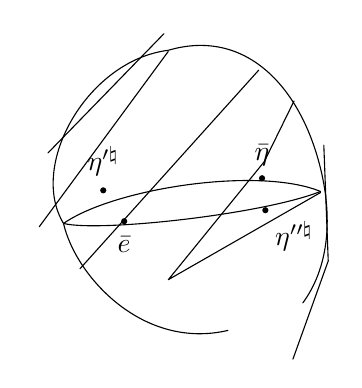
\begin{tikzpicture}[x=.014cm,y=-.014cm,line cap=round,line join=round]
\draw (34,182) .. controls (2,129) and (56,34) .. (129,25)
 .. controls (197,5) and (248,55) .. (267,132)
 .. controls (279,181) and (273,224) .. (251,254);
\draw (34,182) .. controls (45,230) and (106,297) .. (183,279);
\draw (34,182) .. controls (80,150) and (211,130) .. (267,153);
\draw (34,182) .. controls (66,190) and (214,174) .. (267,153);
\fill (70,152) circle (2.8);
\fill (214,141) circle (2.8);
\fill (89,180) circle (2.8);
\fill (217,170) circle (2.8);
\node[above] at (70,148) {$\unsure{\eta'^\natural}$};
\node[above] at (214,139) {$\bar\eta$};
\node[below] at (89,185) {$\bar e$};
\node[below right] at (217,172) {$\unsure{\eta''^\natural}$};
\draw (20,118)--(125,10) (12,185)--(129,26)
 (49,223)--(211,43);
\draw (243,71)--(216,126)--(129,233)--(267,154);
\draw (242,305)--(274,216)--(270,111);
\end{tikzpicture}}
\figure{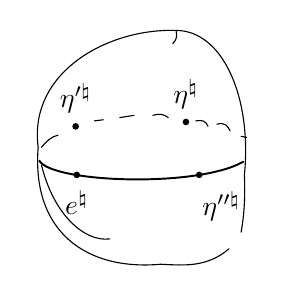
\begin{tikzpicture}[x=.014cm,y=-.014cm,line cap=round,line join=round]
\draw (14,126) .. controls (5,58) and (77,18) .. (139,20)
 .. controls (181,20) and (208,80) .. (201,151)
 .. controls (202,177) and (200,191) .. (198,203);
\draw (187,218) .. controls (167,235) and (147,233) .. (125,232)
 .. controls (57,238) and (8,202) .. (14,126);
\draw (17,126) .. controls (21,121) and (26,116) .. (32,115);
\draw (65,102)--(73,101) (88,99)--(101,97);
\draw (118,97) .. controls (124,95) and (128,96) .. (132,99);
\draw (157,102) .. controls (163,101) and (166,102) .. (168,107);
\draw (176,105) .. controls (184,103) and (186,107) .. (188,111);
\draw (198,116)--(203,117);
\draw[line width=.7pt] (15,138) .. controls (26,158) and (158,163) .. (200,139);
\draw[thin] (139,20) .. controls (140,25) and (140,28) .. (136,32);
\draw[thin] (17,142) .. controls (28,187) and (56,212) .. (79,209);
\fill (48,107) circle (3);
\fill (148,103) circle (3);
\fill (49,151) circle (3);
\fill (160,151) circle (3);
\node[above] at (48,104) {$\eta'^\natural$};
\node[above] at (148,100) {$\eta^\natural$};
\node[below] at (49,157) {$e^\natural$};
\node[below right] at (154,158) {$\eta''^\natural$};
\end{tikzpicture}}

\margin{6}

\scanpage{8}

\begin{center}
U N I V E R S I T E\\
DES SCIENCES ET TECHNIQUES\\
DU LANGUEDOC\\
\texttt{\_\_\_\_\_\_\_\_\_\_\_\_}

Service de la Scolarité\\
MA/GJ\\
Diffusion : Liste A\\
N° : 4679
\end{center}

Montpellier, le 20 octobre 1983

\begin{center}
AVIS DE SOUTENANCE D'UNE THESE DE DOCTEUR INGENIEUR\\
\texttt{\_\_\_\_\_\_\_\_\_\_\_\_\_\_\_\_\_\_\_\_\_\_\_\_\_\_\_\_\_\_\_\_\_\_\_\_\_\_\_\_\_\_\_\_\_\_\_\_\_\_\_\_}

AUTOMATIQUE\\
\texttt{\_\_\_\_\_\_\_\_\_\_\_}
\end{center}

\uline{Nom et prénom du candidat} : SITOHANG Benhard

\uline{Titre de la thèse} : LINAIRE : SYSTEME DE GESTION DE BASES DE DONNEES RELATIONNELLES SUR MICRO-ORDINATEUR.

\uline{Date, heure et lieu de soutenance prévus:} 28 OCTOBRE 1983 à 14h30 - CRIG USTL

\uline{Nom du Directeur de thèse} : Monsieur le Professeur B. FILLIATRE

\uline{Désignation du laboratoire où la thèse est préparée} : CRIG USTL

\uline{Résumé de la thèse} :

La conception et la réalisation d'un Système de Gestion de Bases de Données Relationnelles sur micro-ordinateur, que nous avons baptisé ``LINAIRE'', est le sujet de cette thèse.

Nous mettons l'accent sur trois points principaux :

1. BOUCLE MULTI-NIVEAUX ; c'est une technique du traitement de données, permettant d'éviter l'utilisation des relations intermédiaires comme résultats des opérateurs relationnels, ce qui serait particulièrement pénalisant pour un micro-ordinateur possédant une mémoire centrale limitée.

2. STRUCTURE INTERNE DE LA BASE ; elle est multiple, afin de préserver au mieux les performances tout en offrant en particulier la possibilité d'accélérer le traitement de l'opérateur relationnel ``équi-joint''.

3. L'adaptation sur un micro-ordinateur du langage de manipulation de QUERY-BY-EXAMPLE (langage de haut niveau, interactif, et tabulaire).

\uline{Durée approximative des recherches ayant abouti à la thèse} : 2 ans

\uline{Composition du jury proposé} :

\begin{tabular}{ll}
MM. & FILLIATRE B.\\
& CHEIN M.\\
& PICHAT E.\\
& PIROTTE A.\\
& PRUNET F.
\end{tabular}

\begin{center}
P. le Secrétaire Général,\\
l'Attachée Principale d'Administration Scolaire\\
et Universitaire,

\unsure{A. Gentil}\\[-1ex]
\hspace*{2em}\rule{3em}{0.3pt}

A. GENTIL
\end{center}

\margin{7}

\scanpage{9}
\mspage{3}

B) Courbes \inserted{ell.} anharmoniques de type hexagonal.

La catégorie de ces courbes équivalente \unsure{:|;|à} celle des hexagones orientés, i.e. des torseurs $S$ sous
\[
\begin{aligned}
\mathbb Z/6\mathbb Z&\simeq\mu_6(\mathbb C)\simeq
\text{groupe des}\\
&\qquad\text{unités \inserted{alg.} de }Q(\underset{\zeta}{\underline{\sqrt[3]{1}}})\\
&\simeq\text{groupe des unites \unsure{de}}\\
&\qquad\text{\uline{de}}\ \deleted{\mathbb Z[\zeta]=\mathbb Z(T]/}\\
&\qquad\mathbb Z[\zeta]=\mathbb Z[T]/(1+T+T^2)\\
&\qquad(\zeta=\exp 2i\pi/3)
\end{aligned}
\]

\figure{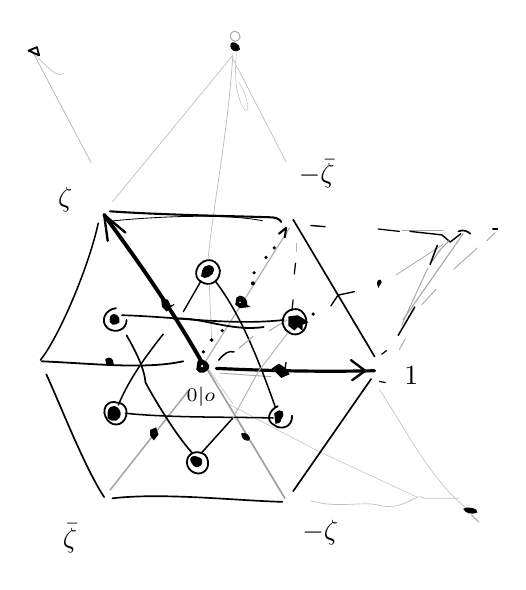
\begin{tikzpicture}[x=.015cm,y=-.015cm,line cap=round,line join=round]
\draw[gray!60,line width=.25pt] (171,917)--(221,1012);
\draw[gray!50,line width=.25pt] (174,921).. controls (183,930) and (193,941) .. (197,936);
\draw[gray!50,line width=.25pt] (239,1045)--(340,922)--(386,1011);
\draw[gray!55,line width=.25pt] (341,920).. controls (337,985) and (324,1050) .. (320,1093);
\draw[gray!45,line width=.22pt] (344,919).. controls (341,947) and (347,962) .. (351,967)
 .. controls (357,971) and (352,952) .. (346,944);
\draw[gray!50,line width=.25pt] (321,1114)--(323,1162);
\draw[gray!45,line width=.25pt] (320,1186)--(341,1216);
\draw[gray!45,line width=.22pt] (337,1216)--(413,1256)--(497,1295);
\draw[gray!45,line width=.25pt] (465,1204).. controls (487,1236) and (507,1280) .. (542,1307);
\draw[gray!50,line width=.25pt] (407,1298).. controls (429,1305) and (452,1298) .. (465,1302)
 .. controls (487,1307) and (496,1290) .. (503,1296)--(532,1296);
\draw[line width=.55pt] (227,1063).. controls (219,1100) and (194,1159) .. (178,1179);
\draw[line width=.6pt] (183,1191).. controls (195,1217) and (215,1269) .. (232,1295);
\draw[line width=.6pt] (239,1296).. controls (282,1291) and (344,1298) .. (383,1299);
\draw[line width=.6pt] (392,1290)--(458,1195);
\draw[line width=.6pt] (461,1176)--(392,1060);
\draw[line width=.75pt] (237,1053).. controls (280,1056) and (339,1057) .. (371,1058)
 .. controls (377,1058) and (380,1059) .. (382,1062);
\draw[line width=.3pt] (240,1061).. controls (282,1057) and (336,1055) .. (366,1061);
\draw[line width=.65pt] (179,1180).. controls (225,1182) and (266,1187) .. (299,1180);
\draw[gray!70,line width=.55pt] (237,1289)--(304,1204);
\draw[gray!60,line width=.45pt] (316,1183)--(389,1067);
\draw[gray!75,line width=.6pt] (320,1188)--(385,1296);
\draw[line width=1.4pt] (316,1183).. controls (286,1130) and (258,1092) .. (232,1056);
\draw[line width=.85pt] (235,1078)--(232,1056)--(250,1071);
\draw[line width=1.15pt] (327,1186).. controls (371,1188) and (413,1189) .. (461,1188);
\draw[line width=.85pt] (441,1179)--(453,1188)--(442,1196);
\draw[gray!65,line width=.35pt] (330,1190)--(373,1193);
\draw[line width=.75pt] (380,1072)--(386,1067)--(385,1075);
\draw[line width=.5pt] (314,1112)--(299,1138);
\draw[line width=.55pt] (282,1157).. controls (263,1181) and (252,1198) .. (244,1217);
\draw[line width=.55pt] (326,1112).. controls (345,1137) and (359,1168) .. (377,1219);
\draw[line width=.55pt] (250,1224).. controls (288,1228) and (341,1227) .. (375,1228);
\draw[line width=.6pt] (247,1141).. controls (290,1142) and (340,1150) .. (384,1145);
\draw[line width=.65pt] (291,1144).. controls (314,1142) and (338,1155) .. (367,1151);
\draw[line width=.6pt] (251,1158).. controls (259,1172) and (266,1186) .. (267,1198)
 .. controls (274,1211) and (291,1240) .. (306,1257);
\draw[line width=.55pt] (314,1258)--(341,1228);
\draw[gray!60,line width=.35pt] (341,1228)--(363,1188)--(389,1154);
\draw[line width=.55pt] (329,1179).. controls (334,1173) and (337,1171) .. (342,1172);
\draw[gray!65,line width=.4pt] (346,1169)--(358,1159);
\draw[gray!65,line width=.4pt] (372,1154)--(387,1145);
\draw[line width=.45pt] (391,1137)--(392,1128);
\draw[line width=.45pt] (393,1106)--(394,1097);
\draw[gray!55,line width=.3pt] (395,1080)--(395,1087);
\draw[line width=.5pt] (424,1133)--(430,1124)--(444,1121);
\draw[gray!65,line width=.3pt] (479,1107)--(519,1081);
\draw[line width=.45pt] (464,1068)--(482,1070);
\draw[gray!70,line width=.3pt] (484,1069)--(519,1069);
\draw[line width=.5pt] (491,1070)--(518,1073)--(525,1079)--(534,1072);
\draw[gray!75,line width=.4pt] (524,1078)--(517,1085)--(510,1095);
\draw[line width=.55pt] (508,1098)--(514,1082);
\draw[gray!70,line width=.35pt] (484,1149)--(506,1101);
\draw[line width=.55pt] (481,1158)--(495,1134);
\draw[gray!70,line width=.4pt] (485,1145)--(536,1072);
\draw[line width=.6pt] (532,1070).. controls (536,1068) and (540,1070) .. (542,1072);
\draw[gray!65,line width=.35pt] (482,1170)--(487,1161);
\draw[gray!65,line width=.35pt] (501,1132)--(513,1119);
\draw[gray!65,line width=.35pt] (528,1102)--(548,1084);
\draw[gray!65,line width=.35pt] (556,1078)--(563,1071);
\draw[line width=.45pt] (561,1068)--(565,1068);
\draw[line width=.5pt] (407,1065)--(419,1066);
\draw[line width=.45pt] (467,1174)--(471,1171);
\draw[line width=.45pt] (465,1197)--(470,1198);
\draw[line width=.65pt] (168,917)--(175,914)--(177,921)--cycle;
\draw[gray!65,line width=.4pt] (339,906).. controls (338,898) and (347,899) .. (347,906)
 .. controls (345,910) and (341,910) .. (339,906);
\fill (339,911).. controls (341,908) and (347,911) .. (347,916)
 .. controls (344,919) and (338,918) .. (339,911);
\fill (536,1305).. controls (540,1302) and (549,1305) .. (548,1308)
 .. controls (543,1310) and (538,1309) .. (536,1305);
\draw[gray!65,line width=.4pt] (543,1310)--(549,1316);
\draw[line width=.65pt] (330,1103).. controls (330,1111) and (324,1116) .. (317,1114)
 .. controls (307,1111) and (309,1101) .. (314,1097)
 .. controls (320,1092) and (328,1094) .. (330,1103);
\fill (315,1103).. controls (317,1097) and (325,1097) .. (325,1103)
 .. controls (325,1107) and (317,1112) .. (314,1108)--cycle;
\draw[line width=.65pt] (251,1145).. controls (251,1153) and (242,1157) .. (235,1152)
 .. controls (228,1146) and (233,1136) .. (242,1135);
\fill (237,1142).. controls (241,1137) and (246,1142) .. (245,1147)
 .. controls (242,1150) and (235,1151) .. (237,1142);
\draw[line width=.65pt] (403,1144).. controls (405,1154) and (396,1160) .. (389,1156)
 .. controls (379,1150) and (383,1137) .. (392,1136)
 .. controls (398,1135) and (401,1138) .. (403,1144);
\fill (388,1142)--(396,1141)--(401,1144)--(405,1147)--(400,1149)
 --(400,1154)--(396,1151)--(393,1154)--(388,1150)--cycle;
\draw[line width=.65pt] (251,1223).. controls (251,1233) and (241,1237) .. (235,1230)
 .. controls (228,1221) and (235,1212) .. (243,1215)
 .. controls (248,1215) and (251,1219) .. (251,1223);
\fill (235,1223).. controls (236,1215) and (245,1217) .. (246,1224)
 .. controls (246,1230) and (240,1233) .. (235,1228)--cycle;
\draw[line width=.65pt] (391,1226).. controls (392,1235) and (382,1239) .. (376,1234)
 .. controls (368,1230) and (372,1221) .. (379,1218);
\fill (376,1224).. controls (383,1218) and (386,1224) .. (382,1229)
 .. controls (382,1232) and (379,1233) .. (377,1233)--cycle;
\draw[line width=.65pt] (320,1265).. controls (321,1273) and (313,1278) .. (306,1273)
 .. controls (299,1268) and (302,1257) .. (310,1257)
 .. controls (317,1257) and (319,1260) .. (320,1265);
\fill (305,1264).. controls (304,1258) and (314,1260) .. (315,1264)
 .. controls (316,1270) and (308,1273) .. (305,1264);
\fill (233,1178).. controls (237,1175) and (240,1178) .. (240,1182)
 .. controls (238,1185) and (233,1185) .. (233,1178);
\fill (280,1126)--(286,1128)--(289,1134)--(285,1138)--(281,1134)--cycle;
\draw[line width=.45pt] (286,1135)--(291,1132);
\fill (344,1126).. controls (347,1122) and (354,1126) .. (353,1132)
 --(356,1134)--(347,1135)--(343,1132)--cycle;
\fill[white] (347,1130) circle[radius=.35pt];
\fill (374,1186)--(380,1182)--(386,1186)--(389,1191)--(382,1194)--cycle;
\draw[line width=.5pt] (385,1187)--(386,1181);
\fill (271,1238)--(276,1236)--(278,1242)--(274,1247)--(271,1243)--cycle;
\fill (348,1241).. controls (352,1239) and (357,1244) .. (355,1247)
 .. controls (352,1248) and (348,1246) .. (348,1241);
\fill (311,1180).. controls (312,1177) and (319,1178) .. (321,1184)
 .. controls (321,1190) and (312,1192) .. (310,1187)--cycle;
\fill[white] (315,1184) circle[radius=.45pt];
\fill (316,1172) circle[radius=.65pt];
\fill (323,1162) circle[radius=.7pt];
\fill (332,1154) circle[radius=.65pt];
\fill (358,1114) circle[radius=.75pt];
\fill (359,1105) circle[radius=.65pt];
\fill (369,1092) circle[radius=.65pt];
\fill (376,1084) circle[radius=.65pt];
\fill (409,1140) circle[radius=.65pt];
\fill (463,1114).. controls (463,1110) and (467,1110) .. (467,1113)
 --(464,1118)--cycle;
\node at (199,1043) {$\zeta$};
\node at (412,1021) {$-\bar\zeta$};
\node at (492,1192) {$1$};
\node at (203,1330) {$\bar\zeta$};
\node at (415,1325) {$-\zeta$};
\node[font=\scriptsize] at (314,1210) {$\unsure{0|o}$};
\end{tikzpicture}}

\deleted{\unsure{On pourra|On pose}} \inserted{On pose}
\[
\mathbb E\ell_1\unsure{\deleted{(S))}|\deleted{(S)}}\simeq\mathbb C/\mathbb Z[\zeta]
\]
\[
\mathbb E\ell_1(S)\simeq\mathbb E\ell_1\mathbin{\wedge}_{\mathbb Z/6\mathbb Z}S
\]

\uline{Construction} On réalise l'hexagone comb. $S$ euclidiennement (canonique), dans \unsure{vectoriel} euclidien $V_S$, \deleted{\unsure{centre}} \inserted{origine} etant le barycentre de $S$. On désigne par $V_S$ le \deleted{\unsure{lattice}} \inserted{réseau} engendré par $S$, et
\[
X_S=\mathbb E\ell_1(S)\simeq V_S/\Gamma_S
\]
La structure euclidienne \uline{orientée} de $V_S$ definit la structure complexe de $X_S$.

\margin{8}

\scanpage{10}

\noindent
\begin{minipage}[t]{0.44\linewidth}
\centering
U N I V E R S I T E\\
DES SCIENCES ET TECHNIQUES\\
DU LANGUEDOC\\
\textasciicircum\textasciicircum\textasciicircum\textasciicircum\textasciicircum\textasciicircum\textasciicircum\textasciicircum\textasciicircum\textasciicircum\textasciicircum\textasciicircum\textasciicircum
\end{minipage}\hfill
\begin{minipage}[t]{0.53\linewidth}
\raggedleft
\vspace{\baselineskip}
Montpellier, le 18 octobre 1983
\end{minipage}

Service de la Scolarité

\begin{tabular}{@{}ll@{}}
Diffusion : & Liste A\\
AM/gs & N° 4570
\end{tabular}

\begin{center}
AVIS DE SOUTENANCE D'UNE THESE DE DOCTEUR-INGENIEUR

``ECOLOGIE GENERALE ET APPLIQUEE option ECOLOGIE TERRESTRE''

\texttt{============================================================}
\end{center}

\uline{NOM et prénom du candidat} : MOUFADDAL Mohamed

\uline{Titre de la thèse} : ``CONTRIBUTION A L'ETUDE DES POSSIBILITES D'EXTENSION DU CEDRE DE L'ATLAS EN DEHORS DE SON AIRE ACTUELLE''

\uline{Date, heure et lieu de soutenance p\unsure{r}évus} : Le 28 octobre 1983 à 14 heures à l'Institut de Botanique

\uline{Nom du directeur de thèse} : M. GODRON Michel

\uline{Désignation du laboratoire où la thèse est préparée} : Centre d'Etudes Phytosociologiques et écologiques Louis Emberger(CNRS)

\uline{Aanlyse de l'ouvrage} : L'objet de cette étude étant de cerner les possibilités d'extension du Cèdre (\uline{Cedrus atl\unsure{a}}n\uline{tica} Manetti) en dehors de son aire actuelle, il a fallu, après une analyse de l'histoire de répartition du Cèdre, préciser les facteurs climatiques responsables de la distribution actuelle.

Les régions où l'introduction du Cèdre est possible, sont déterminées à partir de l'étude climatique de stations situées à l'intérieur et à l'extérieur de l'aire du Cèdre, et par une étude écologique et dendromé-\\
trique comparative de quelques plantations.

\uline{Durée approximative des recherches ayant abouti à la thèse} : 5 ans

\uline{Composition du jury proposé} : \begin{tabular}[t]{ll}
MM. & GODRON M.\\
& BEDEL J.\\
& SCHOENENBERGER A.\\
& ROMANE F.\\
& DAGET Ph.
\end{tabular}

\begin{flushright}
P/ le Secrétaire Général,\\
l'Attachée principale d'administration\\
scolaire et universitaire,

\handwritten{\uline{\unsure{A. Gentil}}}

\uline{A. GENTIL}
\end{flushright}

\margin{9}

\scanpage{11}
\mspage{4}

Le groupe $\mathbb Z/6\mathbb Z$ opère transitivement sur
$({}_2X_S)\setminus\{0\}$ \unsure{(}car $\pm1$ opère trivial\textsuperscript{t} - donc
${}_2X_S\setminus\{0\}$ est un torseur sous
$(\mathbb Z/6\mathbb Z)/\pm1\simeq\mathbb Z/3\mathbb Z$
(\deleted{\unsure{conj.}} (générateur correspondant
$\unsure{\simeq|=}\,-\bar\zeta\,\unsure{j|\zeta}=\exp\frac{2\pi}{6}$),
\deleted{\unsure{en ce cas}} \inserted{le torseur}
s'identifie : $S/\pm1$, en \unsure{\deleted{\illegible{1}}\inserted{a}}ssociant
\unsure{à|:} chaque $s\in S$ le milieu du rayon
$[0,s]$, ou plutôt son image dans \unsure{\inserted{)}} $X_S$.

L'ens des pts fixes de $\mathbb Z/3\mathbb Z\inserted{\subset\mathbb Z/6\mathbb Z}$ sur $X_S$
est de card 3, il s'obtient en prenant
les barycentres des six triangles
de la subdivision centrale (bibarycentrique)
de l'hexagone (pts cerclés) (tels que
$(1-\bar\zeta)/3$ etc dans le cas \unsure{:} épinglé), ils
se groupent en deux \unsure{paquets|régiments} de 3
mutuellemen\unsure{t} congrus sous $\Gamma$, donc \unsure{donnant|donnent}
deux \unsure{é|e}léments (symétriques) de $X_S$, d'ordre 3,

\margin{10}

\scanpage{12}

\noindent
\begin{minipage}[t]{0.44\linewidth}
\centering
U N I V E R S I T E\\
DES SCIENCES ET TECHNIQUES\\
DU LANGUEDOC\\
\textasciicircum\textasciicircum\textasciicircum\textasciicircum\textasciicircum\textasciicircum\textasciicircum\textasciicircum\textasciicircum\textasciicircum\textasciicircum\textasciicircum\textasciicircum
\end{minipage}\hfill
\begin{minipage}[t]{0.53\linewidth}
\raggedleft
\vspace{\baselineskip}
Montpellier, le 14 octobre 1983
\end{minipage}

Service de la Scolarité

\begin{tabular}{@{}ll@{}}
Diffusion : & Liste A\\
MA/gs & N° 4470
\end{tabular}

\begin{center}
AVIS DE SOUTENANCE D'UNE THESE DE DOCTEUR-INGENIEUR

`` PHYSIQUE\ \ DES MATERIAUX ''

\texttt{====================================================}
\end{center}

\uline{NOM et Prénom du candidat} : GOUDEAU Jacques

\uline{Titre de la thèse} : ``Contraint\unsure{es|\deleted{e}s} de trempe thermique dans des pièces à symétrie de révolution''

\uline{Date, heure et lieu de soutenance prévus} : Le 28 octobre 1983, à 11 heures\\
Salle de l'IREM - Université des Sciences et Techniques du Languedoc

\uline{Nom du Directeur de thèse} : M. ZARZYCKI - M. MAISONNEUVE

\uline{Désignation du Laboratoire où la thèse est préparée} : Laboratoire de Sciences des Matériaux, Mécanique des Milieux continus, Chimie structurale - U.S.T.L.

\uline{Analyse de l'ouvrage} : On étudie l'évolution des champs de température et de contraintes, dans une pièce en verre à symétrie de révolution.

Pour cela on résout par éléments finis un problème de thermovisco-élasticité, avec une loi de comportement de type MAXWELL à coefficients variables en fonction de la température.

On compare les résultats obtenus à ceux d'une méthode optique d'analyse des contraintes ainsi qu'à une méthode industrielle de mésure.

\uline{Durée approximative des recherches ayant abouti à la thèse} : 2 ans

\uline{Composition du jury proposé} : \begin{tabular}[t]{ll}
MM. & ZARZYCKI J.\\
& MAISONNEUVE O.\\
& REGNIER J\\
& FRANCOIS\\
& BOURRET D.
\end{tabular}

\begin{flushright}
P/ le Secrétaire Général,\\
l'Attachée Principale d'Administration\\
Scolaire et Universitaire,

\handwritten{\unsure{A. Gen\uline{til}}}

\uline{A. GENTIL}
\end{flushright}

\margin{11}

\scanpage{13}
\mspage{5}

qui avec l'origine $e$ forment l'ens
des pts fixes de $X_S$. (L'ens
des pts fixes sous $\mathbb Z/6\mathbb Z$ \unsure{est|se} réduit
à $e$.) Les deux pts fixes
sous $\mathbb Z/3\mathbb Z$, distincts de $e$, corres-\newline
pondent aux deux triangles coinscrits
\unsure{de|dans} l'hexagone $S$. (\inserted{les deux} triplets \unsure{des|de}
cotés mutuellement non adjacents.)

D\uline{écompositions cellulaires}\newline
ca\uline{noniques}. Décomposition en
deux faces triangulaires, par trois
arêtes, un seul sommet. Les
faces triangulaires correspondent aux
éléments de $\unsure{(X_S)^\zeta|(X_S^\zeta)}\setminus\{e\}$ (chaque
face en contient un et un seul) i.e.
aux triangles coinscrits de l'hexagone-\newline
Les arêtes correspondent aux trois

\margin{12}

\scanpage{14}

\noindent
\begin{minipage}[t]{0.44\linewidth}
\centering
U N I V E R S I T E\\
DES SCIENCES ET TECHNIQUES\\
DU LANGUEDOC\\
\texttt{\textunderscore\textunderscore\textunderscore\textunderscore\textunderscore\textunderscore\textunderscore\textunderscore\textunderscore\textunderscore\textunderscore\textunderscore}

Service de la Scolarité\\
MA/GJ\\
Diffusion : Liste A\\
N°: 4680
\end{minipage}\hfill
\begin{minipage}[t]{0.53\linewidth}
\raggedleft
\vspace{2\baselineskip}
Montpellier, le 20 octobre 1983
\end{minipage}

\begin{center}
\uline{AVIS DE SOUTENANCE D'UNE THESE DE DOCTORAT DE 3ème CYCLE}

\uline{EVOLUTION ET BIOSYSTEMATIQUE}
\end{center}

\uline{Nom et prénom de la candidate} : CHAKROUN Sa\unsure{\={\i}|ï}da

\uline{Titre de la thèse} : LES VARIATIONS SAISONNIERES DES FORMATIONS SECONDAIRES (BOIS, LIBER, CAMBIUM) DU TRONC DE TROIS ESPECES MEDITERRANEENNES, LE CHENE VERT, L'OLIVIER, ET LE MICOCOULIER : UNE ETUDE HISTOPHYSIOLOGIQUE.

\uline{Date, heure et lieu de soutenance prévus} : 28 Octobre 1983 à 9h30\\
Salle de Cours n°9 - U.S.T.L.

\uline{Nom des Directeurs de thèse} : MM. Charles HEBANT et BONNET

\uline{Désignation du laboratoire où la thèse est préparée} : Laboratoire de Biologie Végétale

\uline{Résumé de la thèse} :

Cette étude concerne l'anatomie, l'histologie et l'histo-\\
chimie des tissus conducteurs secondaires d'\textit{Olea europaea}, de \textit{Quercus ilex}, et de \textit{Celtis australis}.

Le bois et le liber du Chêne et de l'Olivier ont fait l'objet d'une étude structurale approfondie.

Le fonctionnement de la zone cambiale (ainsi que la mise en place de ses dérivés, bois et liber) et l'évolution des réserves amylacées du tronc de ces trois espèces subissent des variations importantes avec le rythme saisonnier, et dans le cas de l'Olivier, avec les alternances de production.

Chez le Chêne et le Micocoulier, la totalité du bois et du liber est différenciée au printemps et en été. Chez l'Olivier, la réactivation cambiale au printemps est plus ou moins précoce selon la charge en fruits ; de plus, seuls les arbres en faible production montrent une reprise d'activité cambiale en automne, cette dernière engendre uniquement du bois.

Chez les trois espèces, la mise en place du liber est initiée plus tardivement que dans le cas du bois. Chez les deux espèces à feuilles persistantes, la zone du liber conducteur ne disparaît jamais, par contre, chez le Micocoulier, à la fin de l'automne et pendant l'hiver, tous les tubes criblés deviennent non conducteurs en accumulant de la callose.

Parallèlement à la réactivation cambiale, on note une hydro-\\
lyse de l'amidon. L'amylogénèse est plus ou moins précoce selon l'espèce observée, et dans le cas de l'Olivier, selon la charge en fruits. Une compétition entre la croissance végé-\\
tative et le développement reproductif de l'Olivier est observée.

Tout au long de l'année, les cellules compagnes et les rayons vasculaires du Chêne et de l'Olivier possèdent une forte activité phosphohydrolasique et respiratoire.

\uline{Durée approximative des recherches ayant abouti à la thèse} : 3 ans

\uline{Composition du jury proposée} :

\begin{tabular}{ll}
MM. & D'AUZAC J.\\
& BONNET A.L.\\
& KAUMAN W.\\
& NABLI M.A\\
& THALER L.\\
& VILLEMUR P.
\end{tabular}

\begin{center}
P. le Secrétaire Général,\\
l'Attachée Principale d'Administration Scolaire\\
et Universitaire,

\handwritten{\unsure{-}\quad\unsure{A. Gen\uline{til\hspace{1em}}}}

A. GENTIL
\end{center}

\margin{13}

\scanpage{15}
\mspage{6}

diagonales de l'hexagone, ou encore aux
trois pts d'ordre $2$ distincts de $e$.

Ici encore on peut ``doubler'' la
décomposition cellulaire, et en \unsure{tirer|trouve}
une autre avec $4$ sommets, \deleted{\unsure{8|6}}\inserted{12} arêtes,
et $8$ faces (triangulaires), qui permet
de mieux comprendre le passage
au quotient par $\pm1$, avec
quatre sommets (dont un sommet
privilégié, correspondant \unsure{:|à} $e$),

\figure{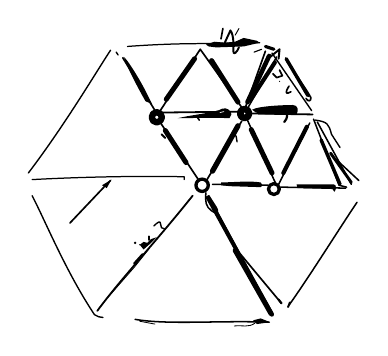
\begin{tikzpicture}[x=.012cm,y=-.012cm,line cap=round,line join=round] \draw[line width=.5pt] (110,48) .. controls (93,74) and (61,128) .. (23,178); \draw[line width=.45pt] (128,44) .. controls (155,42) and (181,41) .. (206,41) -- (268,40); \draw[line width=.45pt] (27,185) .. controls (82,182) and (144,181) .. (188,182) -- (188,185); \draw[line width=.5pt] (27,202) .. controls (41,229) and (63,283) .. (93,328) .. controls (96,330) and (99,331) .. (102,331); \draw[line width=.65pt] (96,324) .. controls (121,290) and (158,251) .. (197,202); \draw[line width=.3pt] (107,310) -- (135,278) -- (151,258); \draw[line width=.55pt] (371,209) .. controls (349,242) and (321,287) .. (299,318); \draw[line width=.7pt] (298,320) -- (300,315); \draw[line width=.55pt] (136,333) .. controls (171,339) and (225,334) .. (278,336); \draw[line width=.3pt] (141,335) -- (157,338); \draw[line width=.3pt] (241,340) .. controls (250,339) and (256,342) .. (263,337); \fill (261,334) -- (269,332) -- (279,336) -- (265,338) -- cycle; \draw[line width=.5pt] (116,50) -- (118,53); \draw[line width=.6pt] (123,56) -- (159,115); \fill (124,55) .. controls (129,59) and (144,84) .. (150,97) -- (154,105) -- (147,102) .. controls (138,86) and (128,67) .. (124,55) -- cycle; \draw[line width=.6pt] (162,113) -- (205,47) -- (250,110); \draw[line width=1.8pt] (169,100) -- (199,57); \draw[line width=1.8pt] (217,59) -- (245,103); \draw[line width=.6pt] (163,125) -- (203,185); \draw[line width=1.8pt] (168,133) -- (190,167); \draw[line width=.65pt] (164,137) -- (168,141); \draw[line width=.6pt] (211,187) -- (249,123); \draw[line width=1.9pt] (218,176) -- (245,128); \draw[line width=.5pt] (241,138) -- (243,139) -- (244,145); \draw[line width=.65pt] (164,114) -- (248,113); \fill (181,120) .. controls (198,116) and (222,114) .. (228,110) .. controls (233,108) and (238,112) .. (238,116) -- (236,120) .. controls (216,119) and (196,120) .. (181,120) -- cycle; \draw[line width=.6pt] (202,119) -- (204,122); \draw[white,line width=.25pt] (226,114) -- (230,113); \draw[line width=.6pt] (253,108) -- (274,49); \draw[line width=1.65pt] (255,103) -- (278,54); \draw[line width=.55pt] (256,108) -- (286,55); \draw[line width=1.5pt] (258,101) -- (284,61); \draw[line width=.7pt] (278,56) -- (289,47) -- (288,57); \draw[line width=1.15pt] (274,44) -- (283,47); \draw[line width=.4pt] (270,47) -- (262,50); \draw[line width=.5pt] (281,51) -- (323,112); \draw[line width=1.25pt] (296,57) -- (319,96); \draw[line width=.6pt] (297,60) .. controls (300,65) and (318,90) .. (322,98) .. controls (323,102) and (319,103) .. (317,99); \draw[line width=.6pt] (289,69) -- (292,75) -- (286,77) -- (282,73); \draw[line width=.6pt] (299,86) .. controls (294,94) and (296,95) .. (301,92); \fill (289,81) circle[radius=.7]; \draw[line width=.65pt] (259,115) -- (324,116); \fill (260,111) .. controls (266,107) and (295,106) .. (303,106) .. controls (309,106) and (309,112) .. (307,116) -- (275,116) -- (264,114) -- cycle; \draw[line width=.8pt] (297,115) .. controls (297,120) and (296,122) .. (294,124); \draw[line width=.55pt] (255,122) -- (283,185) -- (285,189); \draw[line width=1.8pt] (259,132) -- (281,178); \draw[line width=.55pt] (288,190) -- (321,125); \draw[line width=1.5pt] (293,178) -- (318,129); \draw[line width=.55pt] (325,121) -- (352,191) -- (360,193); \draw[line width=1.25pt] (333,143) -- (353,190); \draw[line width=.55pt] (329,124) -- (365,190); \draw[line width=1.05pt] (343,157) -- (365,188); \draw[line width=.55pt] (345,160) -- (373,186); \draw[line width=.5pt] (327,122) .. controls (340,124) and (341,126) .. (344,137) -- (353,151); \draw[line width=.55pt] (218,190) -- (277,191); \fill (227,188) .. controls (239,188) and (257,186) .. (269,188) -- (271,191) -- (269,193) -- (237,192) -- (227,191) -- cycle; \draw[line width=.55pt] (290,193) -- (359,194); \fill (307,190) -- (346,190) .. controls (350,190) and (349,196) .. (347,198) -- (345,195) -- (308,194) -- cycle; \draw[line width=.55pt] (211,199) .. controls (210,208) and (211,214) .. (217,218) .. controls (224,223) and (225,219) .. (221,213) -- (214,202); \draw[line width=1.45pt] (213,204) -- (281,328); \draw[line width=1.8pt] (242,260) -- (280,327); \draw[line width=.6pt] (218,210) -- (246,262) -- (291,316); \draw[line width=.8pt] (288,312) -- (291,316); \draw[line width=.6pt] (67,231) -- (103,193) -- (110,186); \fill (101,191) -- (111,185) -- (106,194) -- cycle; \draw[line width=.8pt] (135,274) -- (144,264); \fill (141,254) -- (145,259) -- (153,252) -- (159,246) -- (153,248) -- (149,252) -- (145,251) -- cycle; \draw[line width=.55pt] (151,249) -- (151,245); \fill (136,252) circle[radius=1.4]; \fill (141,254) circle[radius=.6]; \draw[line width=.5pt] (156,234) .. controls (160,230) and (163,228) .. (163,232) -- (164,236) -- (167,237); \fill (211,42) -- (220,39) -- (231,40) -- (242,39) -- (251,35) -- (265,38) -- (268,40) -- (251,44) -- (222,45) -- (214,44) -- cycle; \draw[line width=.6pt] (227,36) -- (229,25); \draw[line width=.7pt] (231,40) -- (237,27) .. controls (241,33) and (240,43) .. (240,49) .. controls (240,54) and (244,50) .. (246,45); \draw[line width=.35pt] (242,32) -- (246,25); \draw[line width=2.3pt] (159,119) circle[radius=5.4]; \draw[line width=2.4pt] (252,115) circle[radius=4.8]; \draw[line width=1.2pt] (207,191) circle[radius=6.5]; \draw[line width=1.2pt] (283,195) circle[radius=5.8]; \end{tikzpicture}}

six ar\unsure{ê|e}tes les reliant $2:2$ : c'est la
structure tétraédrale \inserted{(orientée)}, avec un sommet
fixé, groupe \unsure{d'automorphismes|d'automorphisme} $\mathbb Z/3\mathbb Z$
(\deleted{\unsure{pourtant}} $\simeq\mathbb Z/6\mathbb Z\,/\pm1$, OK !).

\margin{14}

\scanpage{16}

\begin{center}
U N I V E R S I T E\\
DES SCIENCES ET TECHNIQUES\\
DU LANGUEDOC\\
\textasciicircum\textasciicircum\textasciicircum\textasciicircum\textasciicircum\textasciicircum\textasciicircum\textasciicircum\textasciicircum\textasciicircum\textasciicircum\textasciicircum\textasciicircum
\end{center}

Montpellier, le 14 octobre 1983

Service de la Scolarité

Diffusion : Liste A\\
MA/gs \hfill N° 4469

\begin{center}
AVIS DE SOUTENANCE D'UNE THESE DE DOCTORAT DE 3e CYCLE

`` SCIENCES AGRONOMIQUES\ \ option PHYTOTECHNIE ''\\
\texttt{======================================================}
\end{center}

\uline{NOM et Prénom du candidat} : LECONTE Antoine

\uline{Titre de la Thèse} : ``LA REPRODUCTION SEXUEE DE L'HEVEA BRASILIENSIS\\
(UNE APPROCHE HISTOLOGIQUE ET EXPERIMENTALE)''

\uline{Date, heure et lieu de soutenance prévus} : 27 octobre 1983 à 9h.30 - Salle de cours n°9 - (Bât. administratif ) Université des Sciences et Techniques du Languedoc.

\uline{Nom du Directeur de thèse} : MM. Charles HEBANT - BONNET

\uline{Désignation du laboratoire où la thèse est préparée} : Laboratoire de\\
Biologie végétale - U.S.T.L.\hfill\handwritten{\unsure{\textbackslash}}

\uline{Analyse de l'ouvrage} : L'amélioration génétique de l'Hévéa est entravée par un très mauvais taux de réussite des pollinisations contrôlées.

L'étude histologique montre que le processus reproducteur (gaméto-génèse, fécondation et développement embryonnaire) se déroule normalement. Une exception est signalée : le cas du clone GT 1 dont la stérilité mâle est décrite. La fécondation a lieu moins de 24 heures après la pollinisation.

L'étude expérimentale, menée en Côte d'Ivoire, porte sur les modalités de la floraison et de la fructification en conditions naturelles et artificielles. La majorité des fleurs subissent une élimination naturelle dans un délai de 5 à 15 jours après la pollinisation. Des traitements hormonaux (ANA, chlorure de cobalt) peuvent augmenter significativement le taux de fructification.

Une explication physiologique de la faible fertilité de l'Hévéa est proposée.

\uline{Durée approximative des recherches ayant abouti à la thèse} : 2 ans

\uline{Composition du jury proposé} : \begin{tabular}[t]{ll}
MM. & BONNET\\
& D'AUZAC\\
& HALLE\\
& NICOLAS D.
\end{tabular}

\begin{flushright}
P/ le Secrétaire Général,\\
l'Attachée Principale d'Adminis-\\
tration scolaire et universitaire,

\handwritten{\unsure{;}\quad\unsure{A. Ge\uline{ntil\hspace{1em}}}}

\uline{A. GENTIL}
\end{flushright}

\margin{15}

